\subsection{Changing $\alpha_k$}

\subsubsection{Removing $\alpha_k$}\label{subsubsec:remove-alpha-k}
% Overvej om denne subsubsection er interessant nok at have med i sidste udgave af artiklen, eller om den skal i appendix.
In this experiment we changed $\alpha_k$ from $(1 / (K + 1))$ to $1$ and essentially removed the variable to see what impact it had on the results.
This method is called LightGCN-Ak1 which stands for LightGCN $\alpha_k = 1$.
This will result in the embeddings scaling more than they otherwise would have with $\alpha_k$ as normalization.
As can be seen on \autoref{fig:ndcg-yelp2020-alpha-k} and \autoref{fig:recall-yelp2020-alpha-k} changing $\alpha_k$ decreases performance of LightGCN on the yelp2020 dataset.
In the initial epochs, LightGCN-Ak1 performs better, but quickly starts to decline in performance.
On \autoref{fig:ndcg-amazon-alpha-k} and \autoref{fig:recall-amazon-alpha-k} LightGCN and LightGCN-Ak1 was run on the amazon-book dataset, but can seen that LightGCN still outperforms LightGCN-Ak1.
These results indicates that $\alpha_k$ is an important part of the layer combination for weighted summation, and we will continue our experimentation on trying to optimize $\alpha_k$
\begin{figure}
    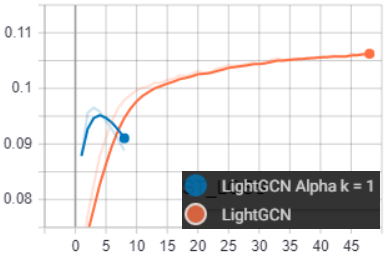
\includegraphics[width=\linewidth]{figures/alpha-k-results/yelp2020-ndcg.png}
    \caption{NDCG@50 of LightGCN and LightGCN-Ak1 on yelp2020}
    \label{fig:ndcg-yelp2020-alpha-k}
\end{figure}
\begin{figure}
    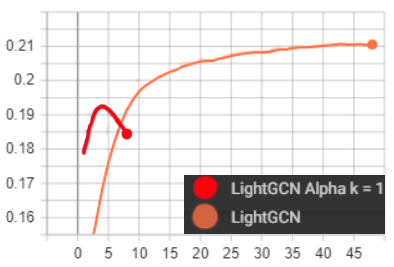
\includegraphics[width=\linewidth]{figures/alpha-k-results/yelp2020-recall.png}
    \caption{Recall@50 of LightGCN and LightGCN-Ak1 on yelp2020}
    \label{fig:recall-yelp2020-alpha-k}
\end{figure}
\begin{figure}
    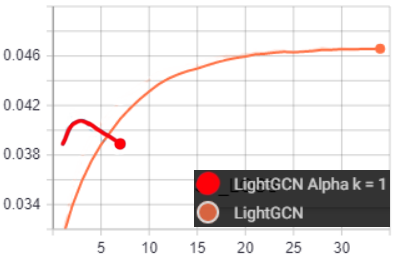
\includegraphics[width=\linewidth]{figures/alpha-k-results/amazon-ndcg.png}
    \caption{NDCG@50 of LightGCN and LightGCN-Ak1 on amazon-book}
    \label{fig:ndcg-amazon-alpha-k}
\end{figure}
\begin{figure}
    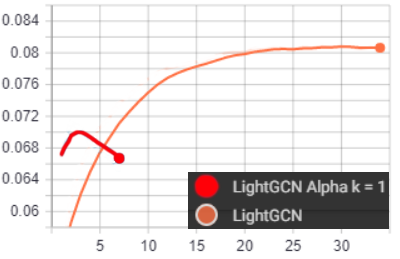
\includegraphics[width=\linewidth]{figures/alpha-k-results/amazon-recall.png}
    \caption{Recall@50 of LightGCN and LightGCN-Ak1 on amazon-book}
    \label{fig:recall-amazon-alpha-k}
\end{figure}
